% ### Uses XeLaTeX ### %
% ### Needs beamer-master ### %
\documentclass[aspectratio=169]{beamer} %. Aspect Ratio 16:9
\usetheme{AI2} % beamerthemeSprace.sty
% DATA FOR FOOTER
\date{2020}
\title{Redes Convolucionais}
\author{}
\institute{Advanced Institute for Artificial Intelligence (AI2)}
\begin{document}
% ####################################
% FIRST SLIDE 						:: \SliTit{This is the Title of the Talk}{A. B. Name}{Sprace}
% SUB-TITLE SLIDE 					:: \SliSubTit{<title>}{<explanation}
% SUB-SUB-TITLE SLIDE				:: \SliSubSubTit{<title>}{<explanation}
% SLIDE WITH TITLE 					:: \SliT{Title}{Content}
% SLIDE NO TITLE 						:: \Sli{Content} 
% SLIDE DOUBLE COLUMN WITH TITLE 	:: \SliDT{Title}{First Column}{Second Column}
% SLIDE DOUBLE COLUMN NO TITLE 		:: \SliD{First Column}{Second Column}
% SLIDE ADVANCED WITH TITLE 			:: \SliAdvT{Title}{Content}
% SLIDE ADVANCED NO TITLE 			:: \SliAdv{Content}
% SLIDE ADVANCED DOUBLE WITH TITLE 	:: \SliAdvDT{Title}{First Column}{Second Column}
% SLIDE ADVANCED DOUBLE NO TITLE 	:: \SliAdvD{First Column}{Second Column}
% SLIDE BLACK						:: \Black{ <Content> }
% SLIDE WHITE						:: \White{ <Content> }
% ITEMIZATION 						:: \begin{itemize}  \iOn{First} \iTw {Second} \iTh{Third} \end{itemize}
% COMMENT TEXT				 		:: \note{<comment>}
% SECTION 							:: \secx{Section} | \secxx{Sub-Section}
% BOLD SPRACE COLOR				:: \bfs{<text>}
% TABLE OF CONTENT					:: \tocitem{<title>}{<content>}
% LEFT ALIGN EQUATION				:: \begin{flalign*}  & <equation> &   \end{flalign*}
% CENTER ALIGN EQUATION	S			:: \begin{gather*} <equations>  \end{gather*}
% SLASH								:: \slashed{<>}
% BAR								:: \barr{<letter>} instead of \bar{<letter>}
% THEREFORE						:: use \portanto (larger and bold}
% 2 or 3 MATH SYMBOLS				:: \overset{<up>}{<down>} &  \underset{<below>}{\overset{<above>}{<middle>}}  
% INSERT TEXT IN FORMULA			:: \ins{<text>}
% EXERCISE							:: \exe{<exercise #>}{<exercise text>}
% SUGGESTED READING BOX			:: \sug{<references>}
% CITATION							:: \cittex{<citation>}
% CITATION DOUBLE COLUMN 			:: \cittexD{<citation>}
% TEXT POSITION						:: \texpos{<Xcm>}{<Ycm>}{<text>} origin = center of slide : x right | y down
% REFERENCE AT BOTTOM  S/D SLIDE		:: \refbotS{<reference>} \refbotD{<reference>}
% HIDDEN SLIDE						:: \hid
% COLOR BOX 						:: \blu{blue} + \red{rec} + \yel{yellow} + \gre{green} + \bege{beige}
% FRAME 							:: \fra{sprace} \frab{blue} \frar{red} + \fray{yellow} + \frag{green}		
% FIGURE 							:: \img{X}{Y}{<scale>}{Figure.png} 
% FIGURE							:: \includegraphics[scale=<scale>]{Figures/.png}
% FIGURE DOUBLE SLIDE NO TITLE		::  \img{-4}{0.5}{<scale>}{Figure.png} % Image 1st half
%									::  \img{4}{0.5}{<scale>}{Figure.png} % Image 2nd half
% FIGURE DOUBLE SLIDE WITH TITLE		::  \img{-4}{0}{<scale>}{Figure.png} % Image 1st half
%									::  \img{4}{0}{<scale>}{Figure.png} % Image 2nd half
% INCLUDING SWF (Flash)				:: \usepackage{media9} and \includemedia >> USE ACROBAT <<
%%%%%%%%%%%%%%%%%%%%%%%%%%%%%%%%%%%%%%%%%%%%%%%%%%
% ###############################################################################
% FIRST SLIDE
\SliTit{Processamento de Imagem}{Advanced Institute for Artificial Intelligence -- AI2}{https://advancedinstitute.ai}


% SLIDE ADVANCED  WITH TITLE
\SliAdvT{Processamento de Imagem}{ 

Agenda

\begin{itemize}
  \iOn{Visão computacional}
  \iOn{Processamento de Imagem}
  \iOn{Análise de Imagem}
  \iOn{Representação de imagem}
  \iOn{Desafios}
\end{itemize}

}

\SliAdvT{Processamento de Imagem}{
A visão computacional procura auxiliar a resolução de problemas
altamente complexos, buscando imitar a cognição humana e a
habilidade do ser humano em tomar decisões de acordo com as
informações contidas na imagem.

}


\SliAdvT{Processamento de Imagem}{

\begin{itemize}
\iOn{O processamento digital de imagens consiste em um conjunto de
técnicas para capturar, representar e transformar imagens com o
auxílio de computador.}

\iOn{O emprego dessas técnicas permite extrair e identificar informações
das imagens e melhorar a qualidade visual de certos aspectos
estruturais, facilitando a percepção humana e a interpretação
automática por meio de máquinas.}
\end{itemize}
}

\SliAdvT{Processamento de Imagem}{
\begin{itemize}
\iOn{A análise/interpretação de imagens visa obter uma descrição que
contenha informação suficiente para distinguir entre diferentes
objetos de interesse, de forma confiável e requerendo o mínimo de
interveção humana.}
\iOn{Certos passos relevantes que envolvem o processamento e a análise de imagens, muitas vezes, á realizada por um operador humano que
detem o conhecimento ou a experiência sobre o domínio da
aplicação.}
\end{itemize}
}

\SliAdvT{Processamento de Imagem}{
\begin{itemize}
\iOn{Análise de imagens capturadas por meio de microscópios ópticos ou
eletrônicos beneficia áreas que variam diversas como biologia por exemplo.}
\iOn{Exemplos de aplicação:}
\iTw{Análise de estruturas em cristalografia}
\iTw{Análise e identificação de espécies de insetos}
\end{itemize}
}

\SliAdvT{Processamento de Imagem}{
A análise de fotografias aéreas ou imagens de satélite permite uma
melhor compreensão da superfície terrestre, auxiliando tarefas como:

\begin{itemize}
\iOn{Estudo de fenômenos naturais como vulcões}
\iOn{Padrões obtidos por copas de árvores}
\iOn{Identificação de áreas de plantio, floresta}
\iOn{Obtenção de características diversas por meio de imagens áreas}
\iOn{Estimativa de caractesíticas de uma propriedade avaliando área construída}
\end{itemize}
}

\SliAdvT{Processamento de Imagem}{ 
Processo de aquisição de uma imagem (Digitalização)

\begin{itemize}
\iOn{Diversos dispositivos podem ser utilizados para realizar aquisição de imagens}
\iTw{Cameras digitais, scanners, satelite, ressonância magnética, etc}
\iOn{As imagens obtidas por tais dispositivos são representadas por meio de um conjunto de pixels}
\iOn{Os dispositivos podem possuir um número variável de canais para obtenção de uma mesma imagem}

\end{itemize}

}
\SliAdvT{Processamento de Imagem}{ 

A representação de uma imagem é feita por meio dos seguintes valores: Altura, Lagura e canais.

\begin{itemize}
\iOn{A altura e lagura definem a quantidade de itens que compõem a imagem que é chamada de pixel}
\iOn{Cada pixel é uma unidade mínima da imagem e pode ser descrito de acordo com diferentes informações chamadas canais}
\end{itemize}

Uma imagem pode ser representada como uma matriz de 3 dimensões sendo altura x largura x canais.
}


\SliAdvT{Processamento de Imagem}{ 
Resolução Espacial
\begin{itemize}
\iOn{A quantidade de pixels presente em uma mesma região da imagem define a resolução.}
\iOn{Quanto mais pixels em uma mesma área da imagem, maior a reolução e portanto, maior o nível de detalhe da imagem}
\iOn{Uma imagem contendo um grande número de pixels não necessariamente possui resolução maior que outra contendo menor número de pixels.}

\iOn{A resolução de uma imagem deve ser escolhida de modo a atender
ao grau de detalhes que devem ser discerníveis na imagem}
\end{itemize}
}


\SliAdvT{Processamento de Imagem}{ 

Exemplos:

\begin{itemize}
\iOn{Uma área de 200 cm2}
\iTw{Se usarmos 10 pixels na dimensão x e 10 pixels na dimensão y, cada pixel vai corresponder a 2 cm2}
\iTw{Se usarmos 20 pixels na dimensão x e 20 pixels na dimensão y, cada pixel vai corresponder a 1 cm2}
\iOn{A resolução influencia a capacidade humana de visualização}
\iOn{A resolução influencia na capacidade de algoritmos realizarem funções automáticas diversas na imagem}
\end{itemize}

}

\SliAdvT{Processamento de Imagem}{ 

Profundidade da imagem

\begin{itemize}
\iOn{Quantidade de variação de valores para cada pixel na representação da imagem}
\iOn{Se utilizamos um número alto de profundidade a imagem possui mais detalhes}
\iOn{Com um número baixo de profundidade a imagem vai possuir menos detalhes}
\iOn{O Processamento da imagem depende de um nível adequado de detalhe}
\iOn{Diminuir a profundidade pode auxiliar em facilitar a manipulação da imagem}
\end{itemize}

}
\SliAdvT{Processamento de Imagem}{ 

\begin{itemize}
\iOn{Uma biblioteca muito popular para processamento de imagem é o opencv}
\iOn{O matplotlib pode ser usado para plotar um array como uma imagem}
\iOn{A seguir mostramos um código elementar para manipulação de imagens}
\end{itemize}

}

\SliAdvT{Processamento de Imagem}{

\begin{lstlisting}
import cv2 as cv \\
import matplotlib.pyplot as plt\\

img = cv.imread('ab5.jpg')\\

plt.imshow(img)

\end{lstlisting}

}


\SliAdvT{Processamento de Imagem}{ 

Desafios relacionados ao processamento de imagens
\begin{itemize}
\iOn{Aumentar ou diminuir}
\iOn{Rotacionar}
\iOn{Correções}
\iOn{Omitir ou realçar detalhes}
\end{itemize}

}

\SliAdvT{Processamento de Imagem}{ 

Aumentar ou diminuir uma imagem

\begin{center}
    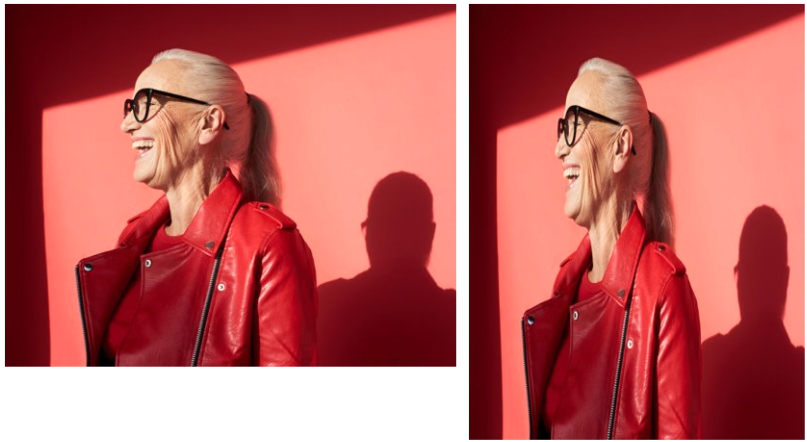
\includegraphics[scale=0.40]{figuras/resize.png}     
\end{center}

}

\SliAdvT{Processamento de Imagem}{ 

\begin{itemize}
\iOn{Quandos mudamos as medidas da imagem, pode ocorrer distorcões}
\iOn{Nesse sentido, é necessário considerar as proporções para fazer um redimensionamento correto}

\end{itemize}

}

\SliAdvT{Processamento de Imagem}{ 

Rotacionar uma imagem

\begin{center}
    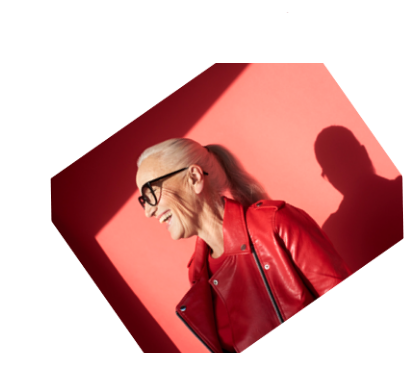
\includegraphics[scale=0.40]{figuras/rotacao.png}     
\end{center}

}

\SliAdvT{Processamento de Imagem}{ 

\begin{itemize}
\iOn{Ao rotacionar uma imagem, é possível que parte da imagem seja cortada}
\iOn{É necessário considerar um novo tamanho que permita incluir a nova imagem completamente}

\end{itemize}

}


\SliAdvT{Processamento de Imagem}{ 

Outras manipulações comuns em uma imagem

\begin{itemize}
\iOn{Recortar uma área de interesse}
\iOn{Incluir um elemento na imagem}
\iTw{Incluir texto}
\iTw{Incluir forma}
\iTw{Incluir outra parte da mesma imagem}
\end{itemize}

}

\SliAdvT{Processamento de Imagem}{ 

Outras operações podem ser realizadas em imagens por meio de filtros:

\begin{itemize}
\iOn{Detectar borda, contornos}
\iOn{Clarear, escurecer}
\iOn{Eliminar ruídos}
\iOn{Transformações morfológicas}
\iOn{Borrar (Blur)}
\end{itemize}

Tais operações auxiliam na identificação de padrões.
}

\SliAdvT{Processamento de Imagem}{ 
\begin{itemize}
\iOn{Filtro é uma operação que é aplicada em todos os pixels de uma imagem, alterando alguns pixels de acordo com certos critérios}
\iOn{Normalmente, a análise de pixels é feito por regiões chamadas vizinhança}
\iTw{A vizinhança de um pixel é definido como o pixel imediatamente acima, abaixo ou aos lados}
\iTw{Normalmente as operações levam em conta a variação de valores da vizinhança do pixel e raramente consideram os pixels isoladamente}
\iOn{O processo de filtragem é feito utilizando matrizes denominadas máscaras, as quais são aplicadas sobre a imagem}

\end{itemize}

}

\SliAdvT{Processamento de Imagem}{ 

\begin{center}
    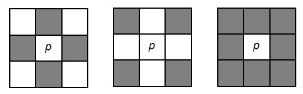
\includegraphics[scale=0.60]{figuras/vizinho.png}     
\end{center}

}
\SliAdvT{Processamento de Imagem}{ 

blur (borrar)

\begin{itemize}
\iOn{Filtro para remover pixels considerados "outlier"}
\iOn{Tais pixels normalmente representam ruídos na imagem}
\iTw{Ruídos podem ser gerados por diversos fatores, como o próprio processo de aquisição}
\end{itemize}

}

\SliAdvT{Processamento de Imagem}{ 

Thresholding

\begin{itemize}
\iOn{Filtro para transformar imagene em imagens binárias}
\iOn{Auxilia em encontrar padrões de contorno na imagem}
\end{itemize}

}

\SliAdvT{Processamento de Imagem}{ 
Filtro de Sobel

\begin{itemize}
\iOn{Calcula o gradiente da intensidade da imagem em cada ponto}
\iOn{Obtendo-se assim uma indicação se a variação de luminosidade em um ponto ocorreu de forma abrupta ou suave}
\iOn{Essa transição claro-escuro ajuda na identificação de contornos}
\end{itemize}

}

\SliAdvT{Processamento de Imagem}{ 

Transformações Morfológicas

\begin{itemize}
\iOn{Erosão: elimina elementos da imagem}
\iOn{Dilatação: aumenta elementos da imagem}
\iTw{Abertura e Fechamento: combina os efeitos da Erosão e Dilatação}
\end{itemize}

}

\SliAdvT{Processamento de Imagem}{

Efeitos da Erosão
\begin{itemize}
\iOn{Diminuir partículas}
\iOn{Eliminar componentes menores que o elemento estruturante}
\iOn{Permitir a separação de componentes conectados}
\end{itemize}
}

\SliAdvT{Processamento de Imagem}{
Efeitos da dilatação
\begin{itemize}
\iOn{Aumentar partículas}
\iOn{Preencher buracos}
\iOn{Conectar componentes próximos}
\end{itemize}
}

\SliAdvT{Processamento de Imagem}{
Identificação de padrões como linhas ou círculos:
\begin{itemize}
\iOn{Hough Lines}
\iOn{Hough Circles}
\end{itemize}
}

\SliAdvT{Processamento de Imagem}{
Filtros do tipo black-hat 

\begin{itemize}
\iOn{Retorna elementos com padrão de tamanho menor e mais escuros que pixels da vizinhança}

\iOn{O tamanho dos elementos extraídos podem ser controlados pelo elemento estruturador}
}
\end{itemize}
}

\SliAdvT{Processamento de Imagem}{
Convolução
\begin{itemize}
\iOn{O OpenCV fornece uma função, cv2.filter2D (), para aplicar uma operação de convolução em um kernel com uma imagem. }
\iOn{Esse processo pode ser generalizado para obter qualquer tipo de padrão em uma imagem}
\end{itemize}
}

\SliAdvT{Processamento de Imagem}{

Camada de convolução em Keras:

\begin{lstlisting}
model.add(layers.Conv2D(32,(5,5),activation='relu',
                                 input\_shape=(28, 28,1)))
\end{lstlisting}

Camada de Pooling: filtro para redução de dimensionalidade
\begin{lstlisting}
model.add(layers.MaxPooling2D((2, 2)))
\end{lstlisting}

\begin{itemize}
\iOn{Normalmente tais camadas são combinadas para realçar padrões que definem características da imagem}
\iOn{Dessa forma, o classificador da rede Neural atua apenas nos padrões encontradas, e não em todos os detalhes }
\end{itemize}
}


\end{document}
